\documentclass[11pt]{article}
\usepackage{amsmath}
\usepackage{cmap}					% поиск в PDF
\usepackage[T2A]{fontenc}			% кодировка
\usepackage[utf8]{inputenc}			% кодировка исходного текста
\usepackage[english,russian]{babel}	% локализация и переносы
\usepackage{textcomp}               % вставка символов
\usepackage[left=2cm,right=2cm,top=2cm,bottom=3cm,bindingoffset=0cm]{geometry} % формат страницы
\usepackage{tipa}                   % фонты и макросы
\usepackage[pdftex]{graphicx}       % вставка графики
\graphicspath{/pictures}
\DeclareGraphicsExtensions{.pdf,.png,.jpg}
\usepackage{fancyhdr}% колонтитул
\usepackage[usenames]{color}
\usepackage{colortbl}





%%% Дополнительная работа с математикой
\usepackage{amsmath,amsfonts,amssymb,amsthm,mathtools} % AMS
\usepackage{icomma} % "Умная" запятая: $0,2$ --- число, $0, 2$ --- перечисление

%% Номера формул
\mathtoolsset{showonlyrefs=true} % Показывать номера только у тех формул, на которые есть \eqref{} в тексте.

%% Шрифты
\usepackage{euscript}	 % Шрифт Евклид
\usepackage{mathrsfs} % Красивый матшрифт

%% Свои команды
\DeclareMathOperator{\sgn}{\mathop{sgn}}

%% Перенос знаков в формулах (по Львовскому)
\newcommand*{\hm}[1]{#1\nobreak\discretionary{}
{\hbox{$\mathsurround=0pt #1$}}{}}


\author{}
\title{}
\date{}

\begin{document}
\tableofcontents
\section{Скалярное поле. Поверхности и линии уровня. Производная по направлению. Градиент скалярного поля.}

\subsection{Определение}
Скалярное поле (скалярная функция) на некотором конечномерном пространстве $V$ - функция, ставящая в соответствие каждой точке из некоторой области этого пространства (область определения) скаляр, то есть действительное или комплексное число. При фиксированном базисе пространства скалярное поле является функцией нескольких переменных, являющихся координатами точки.

Разница между числовой функцией нескольких переменных и скалярным полем заключается в том, что в другом базисе скалярное поле как функция координат изменяется так, что если новый набор переменных представляет ту же точку пространства в новом базисе, то значение скалярной функции не изменяется.

Например, в некотором ортонормированном базисе двумерного векторного пространства скалярная функция имеет вид $f(v)=x^{2}+2y^{2}$ в другом базисе, повернутом на 45 градусов к этому, эта же функция в новых координатах будет иметь вид $f(v)=3x^{2}+3y^{2}-2xy$.
\subsection{Линии и поверхности уровня}
Скалярное поле можно представить графически с помощью поверхностей уровня (также называемой изоповерхностями).

Поверхностью уровня скалярного поля $u=u(x,y,z)$ называется множество точек пространства, в которых функция u принимает одно и то же значение $c$, то есть поверхность уровня определяется уравнением $u(x,y,z)=c$. Изображение набора поверхностей уровня для разных $c$ дает наглядное представление о конкретном скалярном поле, для которого они построены (изображены), кроме того, представление о поверхностях уровня дает определенный дополнительный геометрический инструмент для работы со скалярным полем, который может использоваться для вычислений, доказательства теорем и т. п. Пример: эквипотенциальная поверхность.

Для поля на двумерном пространстве аналогом поверхности уровня является линии уровня. Примеры: изобата, изотерма, изогипса (линия равных высот) на географической карте и прочие изолинии.

Поверхностями уровня для скалярного поля на пространстве большей размерности являются гиперповерхности с размерностью на единицу меньшей, чем размерность пространства.

\subsection{Градиент}

Направление скорейшего возрастания поля $r=u(x,y,z)$ указывает вектор градиента, обозначаемый стандартно:
$\mathbf{grad}\space u$,
или иное обозначение:
$\nabla u$,
с компонентами:
$$\left({\frac  {\partial u}{\partial x}},\ {\frac  {\partial u}{\partial y}},\ {\frac  {\partial u}{\partial z}}\right)$$

Абсолютная величина вектора градиента $u$ есть производная $u$ по направлению скорейшего роста (скорость роста u при движении с единичной скоростью в этом направлении).

Градиент всегда перпендикулярен поверхностям уровня (в двумерном случае — линиям уровня). Исключение — особые точки поля, в которых градиент равен нулю.

\subsection{Производная по направлению}

Рассмотрим дифференцируемую функцию $f(x_{1},\ldots ,x_{n})$ от $n$ аргументов в окрестности точки $\vec {x}=(x_{1}^{0},\;\ldots ,\;x_{n}^{0})$.
 Для любого единичного вектора $\vec {e}=(e_{1},\;\ldots ,\;e_{n})$ определим производную функции
 $f$ в точке $\vec  {x}^{0}$ по направлению $\vec{e}$ следующим образом:

$$ \nabla _{\mathbf {e} }{f}(\mathbf {x} )=\lim _{h\to 0}{\frac {f({\vec {x}}{\,}^{0}+h\cdot {\vec {e}})-f({\vec {x}}{\,}^{0})}{h}}$$
Значение этого выражения показывает, как быстро меняется значение функции при сдвиге аргумента в направлении вектора $\vec{e}$.

Пусть направляющий вектор направления $e$ имеет координаты $e_{1},e_{2}\dots e_{n}$. Тогда имеет место формула:

$$ \nabla _{\mathbf {e} }{f}(\mathbf {x} )={\frac {\partial f}{\partial x_{1}}}e_{1}+\dots +{\frac {\partial f}{\partial x_{n}}}e_{n}$$

На языке векторного анализа эту формулу можно записать иначе. Производную по направлению дифференцируемой по совокупности переменных функции можно рассматривать как проекцию градиента функции на это направление, или иначе, как скалярное произведение градиента на орт направления:

$$\nabla _{\mathbf {e} }{f}(\mathbf {x} )=\nabla f\cdot {\vec {e}}$$
Отсюда следует, что в заданной точке производная по направлению принимает максимальное значение тогда, когда её направление совпадает с направлением градиента функции в данной точке.

\section{Векторное поле. Уравнение векторных линий векторного поля. Дивергенция и ротор векторного поля.}

\begin{center}
\textbf{Векторное поле.}
\end{center}

Векторным полем называется часть пространства (или все пространство), в каждой точке $M$ которого задано какое-либо физическое явление, характеризуемое векторной величиной $\vec{a} = \vec{a}(M)$.

Если в пространстве введена декартова прямоугольная система координат, то задание вектор - функции поля $\vec{a}(M)$ cводится к заданию трех скалярных функций:

$$\vec{a}(M)=a_x(x,y,z)\vec{i}+ a_y(x,y,z)\vec{j} + a_z(x,y,z)\vec{k}$$

Простейшими геометрическими характеристиками векторных полей являются векторные линии и векторные трубки.

\begin{center}
\textbf{Уравнение векторных линий векторного поля.}
\end{center}

Векторными линиями поля $\vec{a} = \vec{a}(M)$ называются линии (кривые), в каждой точке $M$ которых направление касательной совпадает с направлением поля в этой точке.

Векторной трубкой называется поверхность, образованная векторными линиями, проходящими через точки некоторой лежащей в поле замкнутой кривой, не совпадающей (хотя бы и частично) с какой – либо векторной линией.

Для векторного поля $\vec{a}(M)=a_x(x,y,z)\vec{i}+ a_y(x,y,z)\vec{j} + a_z(x,y,z)\vec{k}$ векторные линии описываются системой дифференциальных уравнений:

$$\frac{dx}{a_x(x,y,z)}=\frac{dy}{a_y(x,y,z)}=\frac{dz}{a_z(x,y,z)}$$

Если векторное поле плоское, то при подходящем выборе системы
координат будут выполнены условия $a_x(x,y,z)=a_x(x,y), a_y(x,y,z)=a_y(x,y), a_z(x,y,z)=0$. Тогда будем иметь уравнение:


$$\frac{dy}{dx} = \frac{a_y(x,y)}{a_x(x,y)}, z=const$$	


Известно, что если в некоторой области в трехмерном пространстве
функции $a_x(x,y,z), a_y(x,y,z), a_z(x,y,z)$ непрерывны, имеют непрерывные частные производные первого
порядка и не обращаются в 0, то через каждую точку этой области проходит единственная векторная линия. Это означает, что векторные
линии не пересекаются и не касаются друг друга.

\begin{center}
\textbf{ Дивергенция и ротор векторного поля.}
\end{center}

Дивергенция характеризует отнесенную к единице объема мощность потока векторного поля, “исходящего” из точки $M$. В декартовой системе координат дивергенция вычисляется по формуле:

$$div \vec{a} = (\vec{\nabla}\cdot \vec{a})= \frac{dx}{a_x(x,y,z)}+\frac{dy}{a_y(x,y,z)}+\frac{dz}{a_z(x,y,z)}$$

Свойства дивергенции. Пусть $\vec{a}$ и $\vec{b}$ - векторные поля, $u$ - скалярная функция. Тогда:
\par\bigskip
1) $div(\vec{a}+\vec{b})=div\vec{a}+div\vec{b}$

2) $div(u\cdot\vec{a})=u\, div\vec{a} + (\vec{a}\cdot grad u)$
\par\bigskip

В трехмерном пространстве $rot\vec{a}(M)$ выражается следующим образом:

$$rot\vec{a} = [\vec{\nabla}\times \vec{a}]= \begin{vmatrix} \vec{i} & \vec{j}
& \vec{k}\\
\frac{\partial}{\partial x} & \frac{\partial}{\partial y} & \frac{\partial}{\partial z}\\
a_x & a_y & a_z \end{vmatrix} = \left(\frac{\partial a_z}{\partial y}-\frac{\partial a_y}{\partial z}\right)\vec{i}+
\left(\frac{\partial a_x}{\partial z}-\frac{\partial a_z}{\partial x}\right)\vec{j}+\left(\frac{\partial a_y}{\partial x}-\frac{\partial a_x}{\partial y}\right)\vec{k}$$

Свойства ротора (вихря). Пусть $\vec{a}$ и $\vec{b}$ - векторные поля, $u$ - скалярная функция. Тогда:
\par\bigskip

1) $rot(\lambda\vec{a} + \mu\vec{b}) = \lambda\cdot rot\vec{a} + \mu\cdot rot\vec{b}$

2) $rot(u \cdot \vec{a})=[grad u \times \vec{a}] + u\cdot rot\vec{a}$


\section{Односторонние и двусторонние поверхности. Понятие площади поверхности. Методы вычисления площади поверхности}

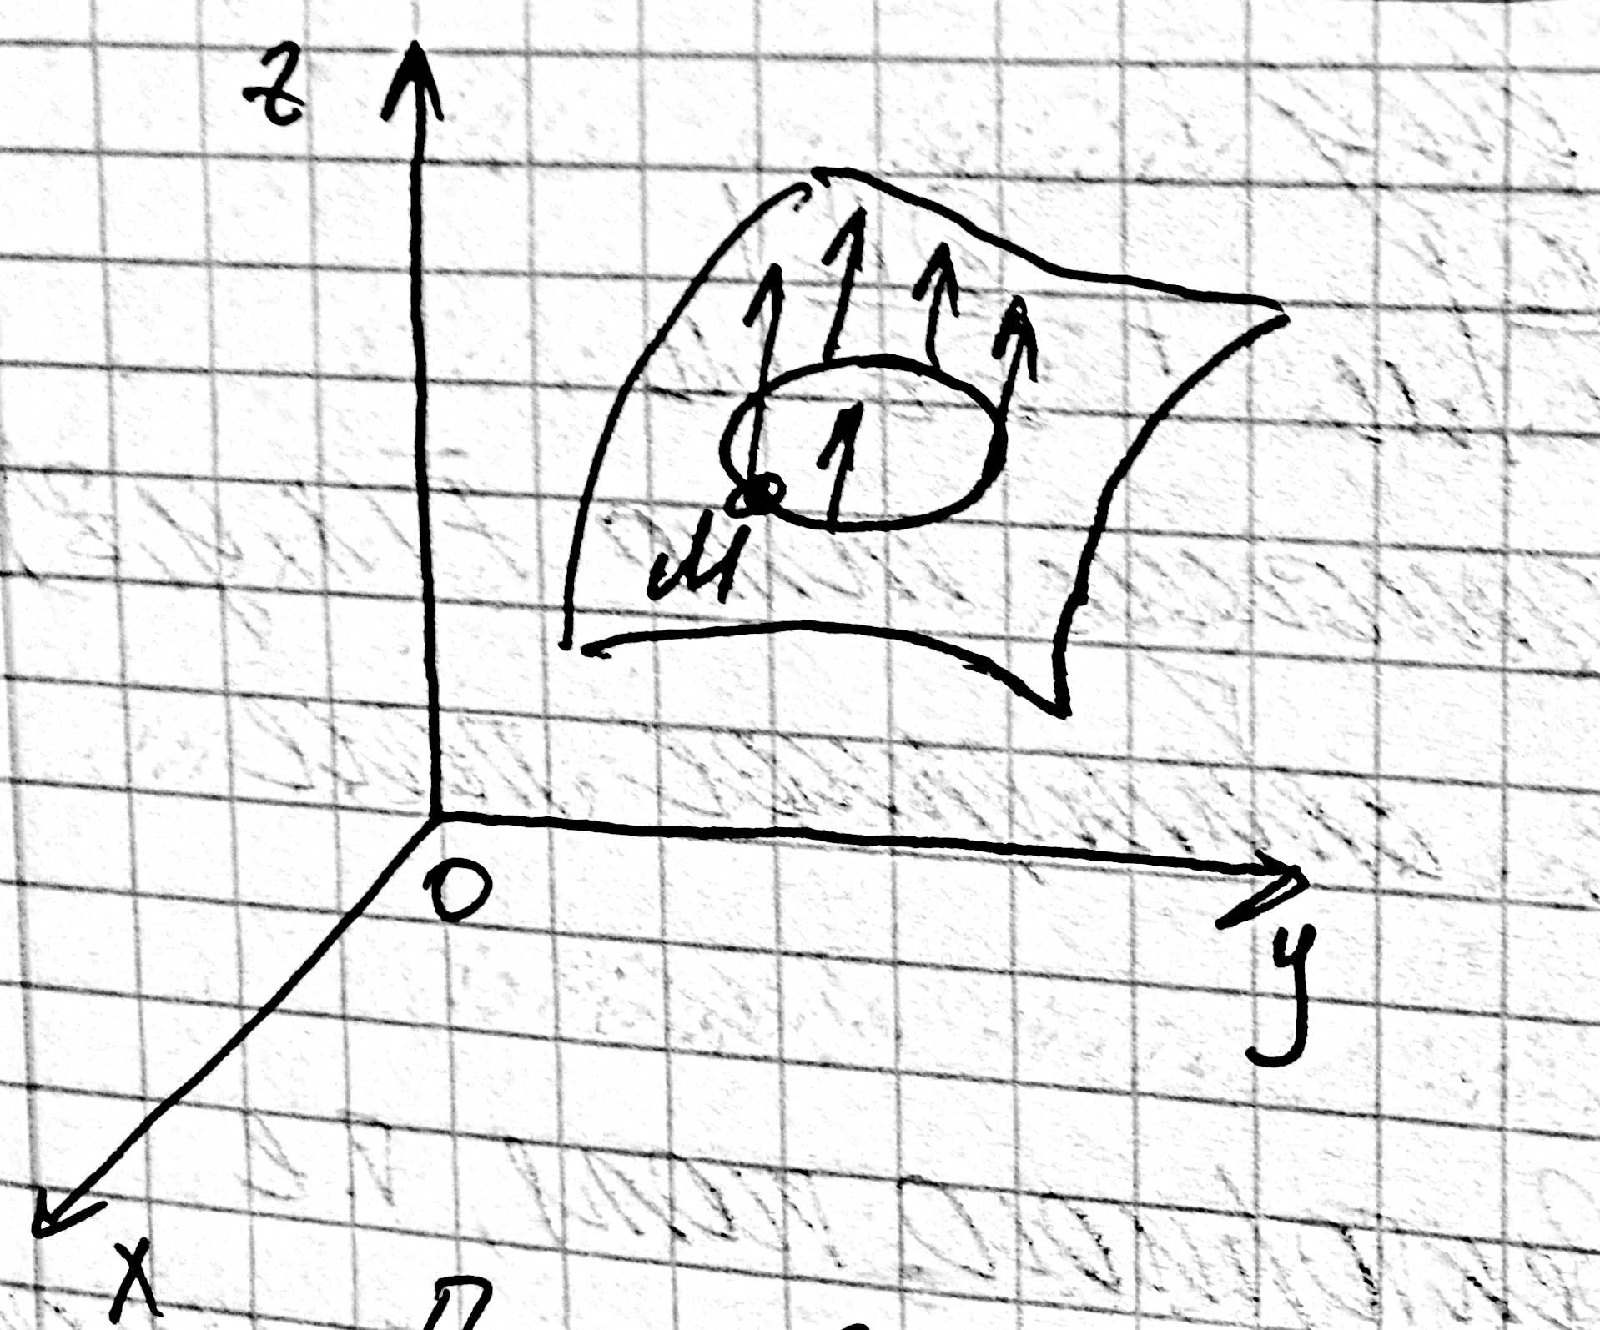
\includegraphics[width=\linewidth]{img/3.jpg}

Пусть в пространстве дана гладкая поверхность $\sigma$. На этой поверхности выберем произвольную точку $M$ и проведем через нее вектор нормали $\overrightarrow{n}$ к поверхности. Через точку $M$ на поверхности $\sigma$ так же проведем произвольный контур, не имеющий общих точек с границей поверхности $\sigma$.

Точку $M$ вместе с вектором нормали будем перемещать по контуру так, чтобы вектор нормали постоянно был перпендикулярен поверхности $\sigma$. 

По возвращении точки $M$ в начальное положение возможны 2 случая: направление $\overrightarrow{n}$ сохранится или поменяется на противоположное. 

Если направление $\overrightarrow{n}$ не поменяется, то поверхность $\sigma$ называется \textbf{двусторонней}.

Если же при обходе контура контура направление $\overrightarrow{n}$ изменится на противоположное, то $\sigma$ - \textbf{односторонняя} 

Двусторонние поверхности называются ориентированными, а односторонние - неориентированными.

Для односторонней поверхности не вводится понятие интеграла 2 рода

\subsection{Понятие площади поверхности}

Пусть $G$ - гладкая (кусочно-гладкая) ограниченная поверхность. Разобьем ее гладкими кривым произвольно на $n$ частей так, чтобы каждая из этих площадок однозначно проецировалась на касательную плоскость, проведенную  в любой точке элементарной площадки.

На каждой элементарной площадке $G_i$ выберем произвольную точку $M_i$ и проведем через эти точки касательные плоскости к поверхности. 

Обозначим через $S_i$ площадь проекции $G_i$ на свою касательную плоскость (эта поверхность ограничена кусочно-гладкими кривыми и потому квадрируема)

Составим сумму: $S(G_i,M_i) = \sum\limits_{i=1}^{n}S_i$\\
Пусть $d_i$ - диаметр $G_i$, $d= d_i (i= 1,2,..,n)$

Если существует предел $\lim\limits_{n\to\infty, d\to 0} S_n = S$, то поверхность называется квадрируемой, а число $S$ - ее площадью
\section{Поверхностные интегралы 1го и 2го рода, определение и методы вычисления}

\begin{center}
	\textbf{Поверхностный интеграл 1-го рода}
\end{center}

Пусть имеется гладкая (кусочно-гладкая) поверхность $\Sigma$ . В точках этой
поверхности задана функция $f(x,y,z)$. Интеграл вида $\iint\limits_\Sigma f(x,y,z) d\sigma$
называется поверхностным интегралом $I$ рода от функции $f(x,y,z)$ по поверхности
$\Sigma$. С физической точки зрения он представляет массу поверхности в точках
которой задана плотность $f(x,y,z)$.
Приведём основные свойства поверхностного интеграла первого рода:

\par\bigskip

\textbf{Свойство 1.} Если $u=f(x,y,z)$ непрерывна на $\Sigma$ , то $f(x,y,z)$ интегрируема.
\par\bigskip
\textbf{Свойство 2.} Линейность. Если $f(x,y,z)$, $g(x,y,z)$ интегрируемы на
$\Sigma$, то их произведение и сумма $\alpha f(x,y,z) + \beta g(x,y,z)$тоже интегрируемы на
$\Sigma$ для любых $\alpha, \beta$.
\par\bigskip
\textbf{Свойство 3.} Для неперекрывающихся гладких (кусочно-гладких) поверхностей $\Sigma_1$ и $\Sigma_2$ при интегрируемой $f(x,y,z)$ будет существовать:
$$\iint\limits_\Sigma f(x,y,z) d\sigma = \iint\limits_{\Sigma_1} f(x,y,z) d\sigma + \iint\limits_{\Sigma_2} f(x,y,z) d\sigma,$$

где $\Sigma=\Sigma_1 \cup \Sigma_2$. Здесь $\Sigma_1$ и $\Sigma_2$ называются неперекрывающимися, если $\Sigma_1 \cap \Sigma_2$ содержит конечное число кусочно-гладких кривых (может быть и пустое). Это свойство 3 называется аддитивностью интеграла $\Sigma$ по области.
\par\bigskip
\textbf{Свойство 4.}  $\iint\limits_\Sigma 1 d\sigma = \Delta\Sigma$ - площадь поверхности $\Sigma$.
\par\bigskip
\textbf{Свойство 5.} Монотонность интеграла. Если $f(x,y,z) \leq g(x,y,z)$ на и функции интегрируемы,то:

$$\iint\limits_\Sigma f(x,y,z) d\sigma \leq \iint\limits_\Sigma g(x,y,z) d\sigma $$

\textbf{Свойство 6.} Если $f(x,y,z)$ интегрируема на $\Sigma$, то $|f(x,y,z)|$ тоже интегрируема на $\Sigma$ и:

$$\left| \iint\limits_\Sigma f(x,y,z) d\sigma\right| \leq \iint\limits_\Sigma |f(x,y,z)| d\sigma. $$

\begin{center}
	\textbf{Сведение поверхностного интеграла 1-го рода к двойному}
\end{center}

\textbf{Случай 1.} Параметрически заданная поверхность. Пусть поверхность $\Sigma$
кусочно-гладкая, задана как $x=x(u,v),\, y=y(u,v),\, z=z(u,v)$, где $(u,v) \in D$ - квадрируемая область и $f(x,y,z)$ - непрерывна на $\Sigma$. Тогда существует:
$$\iint\limits_\Sigma f(x,y,z) d\sigma = \iint\limits_D f(x(u,v), y(u,v), z(u,v)) \sqrt{EG-F^2} dudv.$$
Здесь в интеграле 1-го рода коэффициенты Гаусса $E,G,F$ имеют вид:
$$ E=x_u^{'2}+y_u^{'2}+z_u^{'2}, \,\,\, G=x_v^{'2}+y_v^{'2}+z_v^{'2}, \,\,\, F=x_u^{'}x_v^{'}+y_u^{'}y_v^{'}+z_u^{'}z_v^{'}$$
и поверхностный интеграл 1-го рода существует, если существует двойной интеграл. Оба интеграла существуют, если $f(x,y,z)$ непрерывна на $\Sigma$.

\par\bigskip

\textbf{Случай 2.} Явное задание поверхности $\Sigma$ . Если $\Sigma$ - гладкая поверхность, заданная уравнением $z=z(x,y)$ при $(x,y) \in D$ - квадрируемой области, и $f(x,y,z)$ - ограниченная функция на $\Sigma$ , то интеграл 1-го рода:
$$\iint\limits_\Sigma f(x,y,z) d\sigma = \iint\limits_D f(x,y, z(x,y)) \sqrt{1+z_x^{'2}+z_y^{'2}} dxdy.$$

и существует, если существует двойной интеграл. Для гладкой $\Sigma$ и непрерывной $f(x,y,z)$, оба интеграла существуют одновременно.


В случае поверхности, заданной уравнением $x=x(y,z)$:

$$\iint\limits_\Sigma f(x,y,z) d\sigma = \iint\limits_{D_1} f(x(y,z),y,z) \sqrt{1+x_y^{'2}+x_z^{'2}} dydz,$$

где $(y,z) \in D_1$ - квадрируемая область, а также при $y=y(x,z)$ имеем:
$$\iint\limits_\Sigma f(x,y,z) d\sigma = \iint\limits_{D_2} f(x,y(x,z),z) \sqrt{1+y_x^{'2}+y_z^{'2}} dxdz,$$

для $(x,z) \in D_2$ - квадрируемой области. Отметим, что все эти формулы получаются как частные для параметрически заданной $\Sigma$.

\begin{center}
	\textbf{Поверхностный интеграл 2-го рода}
\end{center}

 Пусть $\Sigma$ - квадрируемая, гладкая двусторонняя поверхность. Фиксируем
одну из её сторон и $P(x,y,z), Q(x,y,z), R(x,y,z)$ - функции, определенные
на $\Sigma$. Тогда интеграл 
$$I=\iint\limits_\Sigma(P\cos\alpha + Q\cos\beta + R\cos\gamma) d\sigma$$
 называется поверхностным интегралом 2-го рода по выбранной стороне поверхности. Здесь
$\cos\alpha, \cos\beta, \cos\gamma$ - косинусы нормали к поверхности, направление которой
согласовано с выбранной стороной. Поверхностный интеграл 2-го рода записывают еще как 
$$I=\iint\limits_\Sigma Pdydz+Qdzdx+Rdxdy.$$ 

При переходе к другой стороне поверхности $I$ меняет знак на противоположный. Отметим, что основные
свойства поверхностного интеграла 2-го рода такие же, как у поверхностного
интеграла 1-го рода. Это линейность относительно подынтегральной функции 
и аддитивность по области при $\Sigma=\Sigma_1\cup \Sigma_2$ для неперекрывающихся поверхностей $\Sigma_1$ и $\Sigma_2$ . Также, если подынтегральная функция непрерывна, то поверхностный интеграл 2-го рода существует.

\begin{center}
	\textbf{Сведение поверхностного интеграла 2-го рода к двойному}
\end{center}

\textbf{Случай 1.} Явное задание поверхности. Пусть гладкая (или кусочногладкая) поверхность $\Sigma$ задана уравнением $z = z(x, y)$ и взята верхняя часть
этой поверхности, а $R(x, y,z)$ - ограниченная на $\Sigma$ функция. Тогда справедливо равенство:

$$\iint\limits_\Sigma R(x, y, z)dxdy = \iint\limits_D R(x, y, z(x, y))dxdy,$$

где $D$ - проекция поверхности $\Sigma$ на плоскость $xOy$. Интеграл слева существует, если существует двойной интеграл. Если же берется нижняя сторона поверхности, то:

$$\iint\limits_\Sigma R(x, y,z)dxdy = - \iint\limits_D R(x, y, z(x, y))dxdy$$

Здесь нижняя и верхняя стороны поверхности $\Sigma$ отличаются противоположным направлением нормали. Отсюда и противоположные знаки в двойном интеграле. Аналогично получаем формулы:

$$\iint\limits_\Sigma P(x, y,z)dydz = \pm \iint\limits_{D_1} P(x(y,z), y, z)dydz$$

$$\iint\limits_\Sigma Q(x, y,z)dzdx = \pm \iint\limits_{D_2} Q(x, y(z,x), z)dzdx$$
Здесь $D_1$ и $D_2$ проекции $\Sigma$ на плоскость $yOz$ и $zOx$ соответственно и оба интеграла – поверхностный и двойной существуют для непрерывных $P,Q, R$.

\par\bigskip

\textbf{Случай 2.} Параметрическое задание поверхностей. Пусть гладкая (или
кусочно-гладкая) поверхность  $\Sigma$ задана равенствами:
$x = x(u, v), y = y(u, v), z = z(u, v), (u, v) \in D$,
а $P = P(x, y, z), Q = Q(x, y, z), R = R(x, y, z)$ ограниченные на  $\Sigma$ функции.

Тогда для выбранной стороны поверхности  $\Sigma$ верно равенство:
$$\iint\limits_\Sigma Pdydz+Qdzdx+Rdxdy = \iint\limits_D (P\cos\alpha + Q\cos\beta + R\cos\gamma)\sqrt{EG-F^2} dudv,$$

где $E,G,F$ - коэффициенты Гаусса, а $\cos\alpha, \cos\beta, \cos\gamma , P,Q,R$ берутся в точке $M = (x(u, v), y(u, v), z(u, v))$. Здесь косинусы нормали имеют вид:

$$ \cos\alpha = \pm \frac{A}{\sqrt{A^2+B^2+C^2}}, \,\,\, \cos\beta = \pm \frac{B}{\sqrt{A^2+B^2+C^2}}, \,\,\, \cos\gamma = \pm \frac{C}{\sqrt{A^2+B^2+C^2}},$$

где величины:

$$A = \begin{vmatrix}
y_u^{'} & z_u^{'} \\
y_v^{'} & z_v^{'}
\end{vmatrix}, \,\,\, B = \begin{vmatrix}
z_u^{'} & x_u^{'} \\
z_v^{'} & x_v^{'}
\end{vmatrix}, \,\,\, C = \begin{vmatrix}
x_u^{'} & y_u^{'} \\
x_v^{'} & y_v^{'}
\end{vmatrix}, \,\,\, \sqrt{A^2+B^2+C^2} = \sqrt{EG+F^2}$$
 
Знаки $\pm$ в косинусах нормали соответствуют
выбранной стороне поверхности $\Sigma$ . При этом имеем значение:
$$\iint\limits_\Sigma Pdydz+Qdzdx+Rdxdy = \pm \iint\limits_D(PA+QB+RC)dudv,$$

где подинтегральные функции в двойном интеграле берутся в точке
$M = (x(u, v), y(u, v), z(u, v))$ и $\pm$ соответствует стороне поверхности.

\section{ Поток векторного поля. Определение потока, свойства и методы вычисления. Физический смысл потока}

\begin{center}
\textbf{Поток векторного поля. Определение потока. Методы вычисления потока.}
\end{center}

Поток векторного поля может быть вычислен в виде поверхностного интеграла, который выражает общее количество жидкости, протекающей в единицу времени через некоторую поверхность в направлении вектора скорости течения жидкости в данной точке. 

\par\bigskip

\textbf{Определение:} Потоком векторного поля  $\vec{a}$ через поверхность $\Sigma$ называется поверхностный интеграл первого рода по $\Sigma$ от скалярного произведения $\vec{a}$ на единичный вектор нормали $\vec{n}_0$ к выбранной стороне поверхности: 

$$\Pi= \lim_{\Delta\sigma_{max}\rightarrow 0} \sum_{i=1}^{n}(\vec{a}(P_i)\cdot\Delta\vec{\sigma}) = \iint\limits_\Sigma(\vec{a}\cdot
d\vec{\sigma})=\iint\limits_\Sigma(\vec{a}\cdot
\vec{n}_0) d\sigma = \iint\limits_\Sigma a_n\, d \sigma$$

\textbf{Примечание:} $a_n$ - проекция поля $\vec{a}$ на нормаль к поверхности $\vec{n}_0$.

\par\bigskip
\textbf{Рассмотрим второй вариант вычисления потока векторного поля:} 

Так как векторное поле $\vec{a}=a_x(x,y,z)\vec{i}+a_y(x,y,z)\vec{j}+a_z(x,y,z)\vec{k}$, а единичный вектор нормали $\vec{n}_0 = (\cos{\alpha}, \cos{\beta}, \cos{\gamma})$,  по формуле скалярного произведения векторов: $\vec{a}\cdot \vec{n}_0 = a_x\cos{\alpha} + a_y\cos{\beta} + a_z\cos{\gamma}$.
Учитывая, что $\cos{\alpha}\, d\sigma = dydz, \, \cos{\beta}\, d\sigma = dzdx, \, \cos{\gamma}\, d\sigma = dxdy$, поток векторного поля можно вычислить и как поверхностный интеграл второго рода:

$$\Pi=\iint\limits_\Sigma a_x dydz + a_y dzdx + a_z dxdy.$$

\begin{center}
	\textbf{Свойства потока.}
\end{center}

1) Линейность:

$$\iint\limits_\Sigma(\alpha \vec{a}_1 + \beta \vec{a}_2, \vec{n}_0)d\sigma = \alpha\iint\limits_\Sigma(\vec{a}_1\cdot
\vec{n}_0) d\sigma + \beta\iint\limits_\Sigma(\vec{a}_2\cdot
\vec{n}_0) d\sigma  $$

2) Аддитивность. Если поверхность $\Sigma$ состоит из нескольких гладких частей $\Sigma_1, \Sigma_2, \Sigma_3, ..., \Sigma_n$, которые могут пересекаться разве что по своим границам, то:
 $$\Pi=\iint\limits_\Sigma(\vec{a}\cdot\vec{n}_0) d\sigma = \sum_{i=1}^{n} \iint\limits_{\Sigma_{i}} (\vec{a}\cdot\vec{n}_0 )d\sigma$$
  
  
3) Поток меняет знак при изменении стороны поверхности. Пусть $\Sigma^+$ – сторона поверхности $\Sigma$, на которой выбрана нормаль $\vec{n}_0$, а $\Sigma^-$ – сторона поверхности $\Sigma$, на которой берется нормаль $-\vec{n}_0$, тогда:

$$\iint\limits_{\Sigma^+}(\vec{a}\cdot
\vec{n}_0) d\sigma = -\iint\limits_{\Sigma^-}(\vec{a}\cdot
\vec{n}_0) d\sigma $$


\begin{center}
	\textbf{Физический смысл потока.}
\end{center}

Пусть $\vec{a}(P_i)$ – поле скоростей некоторой жидкости $\vec{a} = \vec{V}$, а  $\Sigma$ – некоторая поверхность в поле, тогда: $(\vec{a}\cdot d\vec{\sigma}) = (\vec{a}\cdot \vec{n}_0) d\sigma = |\vec{V}|\cos\varphi d\sigma = V_n \cdot d\sigma$ - объём столба жидкости с основанием $d\sigma$ и высотой $V_n$ ($V_n$ - проекция поля $\vec{V}$ на нормаль к поверхности $\vec{n}_0$), т. е. объем
жидкости, протекающей через площадку $d\sigma$ в единицу времени в направлении $\vec{n}_0$. Суммируя по поверхности $\Sigma$ , получаем, что поток жидкости, протекающей через поверхность $\Sigma$ в единицу времени равен:
$$\Pi=\iint\limits_\Sigma(\vec{a} \cdot d \vec{\sigma}).$$


\section{Поток векторного поля через замкнутую поверхность. Теорема Остроградского Гаусса. Инвариантное определение дивергенции}
\section{Линейный интеграл. Понятие линейного интеграла, свойства и методы вычисления. Физический смысл линейного интеграла}
\section{Циркуляция векторного поля. Теорема Стокса. Инвариантное определение ротора. Формула Грина}
\subsection{Циркуляция}
Циркуляцией векторного поля по данному замкнутому контуру $\Gamma$ называется криволинейный интеграл второго рода, взятый по $\Gamma$. По определению

$$C=\oint \limits _{\Gamma }{\mathbf {F} d\mathbf {l} }=\oint \limits _{\Gamma }{(F_{x}dx+F_{y}dy+F_{z}dz)}$$
где $\mathbf {F} =\{F_{x},F_{y},F_{z}\}$ — векторное поле (или вектор-функция), определенное в некоторой области $D$, содержащей в себе контур $\Gamma$, $d\mathbf {l} =\{dx,dy,dz\}$ — бесконечно малое приращение радиус-вектора $\mathbf  {l}$ вдоль контура. 

Окружность на символе интеграла подчёркивает тот факт, что интегрирование производится по замкнутому контуру. Приведенное выше определение справедливо для трёхмерного случая, но оно, как и основные свойства, перечисленные ниже, прямо обобщается на произвольную размерность пространства.

\subsection{Формула Стокса}Циркуляция вектора $\vec F$ по произвольному контуру $\Gamma$ равна потоку вектора $\operatorname {rot} \mathbf {F}$ через произвольную поверхность $S$, ограниченную данным контуром.

$$\oint \limits _{\Gamma }{\mathbf {F} d\mathbf {l} =\iint \limits _{S}{\operatorname {rot} }}\mathbf {F} \cdot \mathbf {n} dS$$,
где $$\operatorname {rot} \mathbf {F} =[\nabla ,\mathbf {F} ]=\left|{\begin{matrix}\mathbf {e} _{x}&\mathbf {e} _{y}&\mathbf {e} _{z}\\{\frac {\partial }{\partial x}}&{\frac {\partial }{\partial y}}&{\frac {\partial }{\partial z}}\\F_{x}&F_{y}&F_{z}\\\end{matrix}}\right|$$— ротор (вихрь) вектора F.


\subsection{Формула Грина}
В случае, если контур плоский, например лежит в плоскости OXY, справедлива теорема Грина

$$\displaystyle \oint \limits _{\Gamma }{(F_{x}dx+F_{y}dy)}=\iint \limits _{\Gamma ^{\circ }}{\left({\frac {\partial F_{y}}{\partial x}}-{\frac {\partial F_{x}}{\partial y}}\right)dxdy}$$
где $\Gamma ^{\circ }$ — плоскость, ограничиваемая контуром $\Gamma$  (внутренность контура).


\subsection{Инвариантное определение ротора}

Пусть $M \in V$. Возьмём малую плоскую площадку $\sigma$, ограниченную контуром  $C$ .
 По теореме Стокса циркуляция по $C$ равна $Z = \oint \limits_C \bar a d\bar r = \iint\limits _{\sigma}\operatorname{rot} \bar a\dot \bar n d\sigma$. 
Считая, что $\operatorname{rot} \bar a$ мало меняется на $\sigma$ и что поверхностный интеграл равен $\operatorname{rot} \bar a(M)\dot \bar n(M)\sigma = |\operatorname{rot} \bar a(M)|cos(\phi)\dot \sigma$, 
получим $Z=|\operatorname{rot} \bar a(M)|cos(\phi)\dot\sigma$.
Будем теперь крутить площадку вокруг точки  $M$, при этом циркуляция меняется вместе с $cos\phi$. Максимальное значение циркуляция получит при $\phi=0$, т.е. когда направления $\operatorname{rot} \bar a(M)$ и $\bar n(M)$ совпадут. Следовательно, $\operatorname{rot} \bar a(M)$ указывает направление, вокруг которого циркуляция максимальна и равна $Z_{\mbox { max } } =|\operatorname{rot} \bar a(M)| \cdot \sigma$

Тогда модуль ротора определяется соотношением:

$$| rot\bar { a } (M)| =\frac { \mbox { Z } _ { \mbox { max } } } { \sigma } $$


\section{Потенциальные и соленоидальные векторные поля. Условия потенциальности векторного поля. Потенциал. Методы вычисления потенциала. Свойства соленоидального поля}
\subsection{Соленоидальное поле}

Векторное поле называется соленоидальным или вихревым, если через любую замкнутую поверхность $S$ его поток равен нулю:

$\int\limits_S \vec a \cdot \vec{ds} = 0$.
Другое определение соленоидального поля: Векторное поле $\vec {a}$ называют соленоидальным, если оно является вихрем некоторого поля $\vec  {b}$, $\vec {a}=\mathrm {rot} \,{\vec {b}}$. При этом векторное поле $\vec  {b}$ называют векторным потенциалом поля $\vec {a}$.

Если это условие выполняется для любых замкнутых S в некоторой области (по умолчанию - всюду), то это условие равносильно тому, что равна нулю дивергенция векторного поля $\vec a$:

$\mathrm {div} \,{\vec {a}}\equiv \nabla \cdot {\vec {a}}=0$
всюду на этой области (подразумевается, что дивергенция всюду на этой области существует). Поэтому соленоидальные поля называют также бездивергентными.

Для широкого класса областей это условие выполняется тогда и только тогда, когда $\vec a$ имеет векторный потенциал, то есть существует некое такое векторное поле $\vec  A$ (векторный потенциал), что $\vec a$ может быть выражено как его ротор:

$\vec {a}=\nabla \times {\vec {A}}\equiv \mathrm {rot} \,{\vec {A}}$.

\subsection{Свойства соленоидального поля}

\begin{itemize}
\item Поток соленоидального векторного поля через поверхность $\sigma$, ограничивающую область $V_{\sigma} \in V$, равен нулю. Это прямое следствие формулы Остроградского.
\item Верно и обратное утверждение: равенство нулю потока через любую замкнутую поверхность $\sigma$ достаточно для соленоидальности поля $\bar a(M)$.

\item Пусть в  $V$  имеется изолированный источник или сток поля. Если поле $\bar a(M)$ соленоидально, то его поток через любую замкнутую поверхность $\sigma$, содержащую этот источник имеет одно и то же значение. Фраза "в  $V$  имеется изолированный источник или сток поля" означает, что область  $V$ , в которой поле соленоидально, неодносвязна - из $V$  выколота точка, в которой находится источник. Так, поле электрической напряжённости, создаваемое зарядом  $q$ ,$\bar E=\frac{q}{r^3}\bar r$, соленоидально всюду, кроме точки $r=0$, в которой расположен источник.
\item Поток соленоидального векторного поля через любое поперечное сечение векторной трубки один и тот же. Это следует из того, что поток через боковую поверхность трубки равен нулю.
\end{itemize}

\subsection{Потенциальное векторное поле}

Потенциальное (или безвихревое) векторное поле в математике — векторное поле, которое можно представить как градиент некоторой скалярной функции координат. \textbf{Необходимым условием} потенциальности векторного поля в трёхмерном пространстве является равенство нулю ротора поля. Однако это условие \textbf{не является достаточным} — если рассматриваемая область пространства не является односвязной, то скалярный потенциал может быть многозначной функцией.

Пусть $\vec {v}$ — потенциальное векторное поле; оно выражается через потенциал $\phi$  как

$\vec  v=\nabla \phi$  (или в другой записи $\vec {v}=\operatorname {grad} \phi $.

Для поля сил и потенциала сил эта же формула записывается как

${\vec  F}({\vec  r},t)=-\nabla U({\vec  r},t)$,
то есть для сил потенциалом $\phi$  является $-U$.

\subsection{Условия потенциальности векторного поля}

Пусть $A = \{A_x, A_y, A_z\}$ – дифференцируемое потенциальное поле, $dr = \{dx,dy,dz\}$ – бесконечно малый вектор смещения их произвольной точки $M(x,y,z)$.

Рассмотрим скалярное произведение векторов  $A$  и  $dr$:
$$A\dot dr = \operatorname{grad} \phi \dot dr = \frac{d\phi}{dx}dx +\frac{d\phi}{dy}dy + \frac{d\phi}{dz}dz$$

Выражение в правой части этого равенства представляет собой полный дифференциал функции . Если частные производные $\frac{d\phi}{dx}, \frac{d\phi}{dy}, \frac{d\phi}{dz}$ являются непрерывными функциями, то смешанные производные $\phi$ не зависят от порядка дифференцирования:

$$\frac{d^2phi}{dxdy} = \frac{d^2phi}{dydx},\frac{d^2phi}{dzdy} = \frac{d^2phi}{dydz}, \frac{d^2phi}{dxdz} = \frac{d^2phi}{dzdx} $$

Учитывая, что частные производные от функции $\phi$ являются координатами вектора $A$, получаем следующие условия потенциальности поля $A$:
$$\frac{\partial A_y}{dx} = \frac{\partial A_x}{dy}$$
$$\frac{\partial A_z}{dx} = \frac{\partial A_x}{dz}$$
$$\frac{\partial A_y}{dz} = \frac{\partial A_z}{dy}$$

\subsection{Вычисление потенциала}

\begin{itemize}
\item Из условий потенциальности:

$$\frac{\partial A_y}{dx} = \frac{\partial A_x}{dy}$$
$$\frac{\partial A_z}{dx} = \frac{\partial A_x}{dz}$$
$$\frac{\partial A_y}{dz} = \frac{\partial A_z}{dy}$$

Отсюда получаем диффуравнения вида:

$$\frac{\partial phi}{dx} = f(x,y,z)$$
$$\frac{\partial phi}{dy} = f(x,y,z)$$
$$\frac{\partial phi}{dz} = f(x,y,z)$$

И решаем их

\item По формуле:

$$\phi(M)-\phi(M^0) = \int\limits_{M^0M}F_xdx + F_ydy + F_zdz = \int\limits_{x_0}x F_xdx+ \int\limits_{y_0}^y F_ydy+  \int\limits_{z_0}^z F_zdz$$

для потенциала векторного поля $\bar F = \{F_x, F_y, F_z\}$ в точке $M$ относительно постоянной точки $M^0$



\end{itemize}








\section{Тригонометрический ряд Фурье. Тригонометрическая система. На-хождение коэффициентов ряда Фурье}
Тригонометрический ряд Фурье — представление произвольной функции $f$ с периодом $\tau$  в виде ряда
$$f(x)=\frac{a_0}{2} + \sum^{\infin}_{n=1} (a_n \cos nx + b_n \sin nx)$$
или используя комплексную запись, в виде ряда:

$$f(x) = \sum\limits_{k=-\infty}^{+\infty} \hat{f}_k e^{ikx}$$

где

$$a_0= \frac{1}{\pi}\int\limits_{-\pi}^{\pi}f(x)dx$$
$$a_n= \frac{1}{\pi}\int\limits_{-\pi}^{\pi}f(x)\cos(nx)dx$$
$$b_n= \frac{1}{\pi}\int\limits_{-\pi}^{\pi}f(x)\sin(nx)dx$$


Тригонометрическая система ортогональна в том смысле что

$$\int\limits_{-\pi}^{\pi}cos(kx)cos(mx)=0, k,m \in N, k\ne m$$
$$\int\limits_{-\pi}^{\pi}sin(kx)sin(mx)=0, k,m \in N, k\ne m$$
$$\int\limits_{-\pi}^{\pi}cos(kx)sin(mx)=0, k,m \in N, k\ne m$$
$$\int\limits_{-\pi}^{\pi}cos^2(kx)=\pi, k \in N$$
$$\int\limits_{-\pi}^{\pi}sin^2(kx)=\pi, k \in N$$



\section{ Кусочно непрерывные и кусочно гладкие функции. 3 леммы (доказать одну)}
\textbf{Кусочно-гладкая функция} — функция, определённая на множестве вещественных чисел, дифференцируемая на каждом из интервалов, составляющих область определения.

\subsection{Кусочно непрерывная функция}

$f(x)$ кусочно непрерывна на $[a,b]$ если она непрерывна на этом отрезке за исключением \textbf{конечного} числа точек(разрывов первого рода).

$x_0$ - \textbf{т. разрыва I рода}, если существуют пределы $\lim_{x\to x_0-0}f(x)$ и $\lim_{x\to x_0+0}f(x)$. Пример такой функции - $sgn(x)$. Если оба предела равны но функция в $x_0$ не определена - разрыв \textbf{устранимый}

\subsection{Кусочно гладкая функция}

$f(x)$ кусочно гладкая на $[a,b]$ если она:
\begin{itemize}
  \item кусочно непрерывна на $[a,b]$
  \item имеет в каждой точке на $[a,b]$ непрерывные производные, за исключением конечного числа точек, где $f(x)$ может не существовать или не быть непрерывной. В этих точках существуют:
  \begin{itemize}
    \item $\lim_{x\to x_0-0}f'(x)$ - левый предел производной
    \item $\lim_{x\to x_0+0}f'(x)$ - правый предел производной
  \end{itemize}
\end{itemize}

\subsection{Лемма о правой производной не существующей в точке функции}

Пусть $f(x)$ дифференцируема в правой полуокрестности точки $x_0$ - $[x_0, x_1]$ и пусть существует 
$$\lim _{x\to x_0+0}f'(x) = f'(x_0+0)$$
тогда 
\begin{itemize}
\item $\exists \lim _{x\to x_0+0}f(x) = f(x_0+0)$
\item $\exists \lim _{\chi \to 0} \frac{f(x_0+\chi)-f(x_0+0)}{\chi} = f'(x_0+0)$
\end{itemize}

Смысл человеческими словами:

Если $f(x)$ не существует в $x_0$, но существует правый предел ее производной, то существует и правый предел самой этой функции. Так же существует и правая производная функции в точке, равная пределу производной справа.

\subsection{Лемма об аппроксимации}

Пусть $f(x)$ непрерывна на $[a,b]$, тогда $\forall \varepsilon>0 \exists e(x): \forall x \in [a,b] |f(x)-e(x)|<\varepsilon, f(a)=e(a), f(b)=e(b)$, $e$ - кусочно гладкая.

По-человечески: любую непрерывную на $[a,b]$ функцию можно аппроксимировать кусочно гладкой функцией так что отличаться они будут на сколь угодно малую величину в каждой из точек отрезка, а на концах - в точках $a$ и $b$ - будут совпадать.

Доказательство:

$f(x)$ - непрерывна на $[a,b]$, значит $\forall \varepsilon >0 \exists \delta >0: \forall x, \forall x' \in [a,b] |x-x'|<\delta \Rightarrow |f(x)-f(x')|<\frac{\varepsilon}2$

По-человечески: разбиваем наш отрезок на очень маленькие отрезки, части функции соответствующие каждой части отрезка заменяем на прямые, чьи значения на краях "кусочков" совпадают с функцией. Полученная функция является кусочно гладкой - она линейна за исключением конечного числа точек. Ну и совпадение на концах отрезка очевидно.




\section{Теорема Дирихле о сходимости суммы ряда Фурье. Сформулировать идею доказательства}

\subsection{Некоторые определения}
Говорят, что функция \(f\left( x \right),\) определенная в интервале \(\left[ {a,b} \right],\) является кусочно непрерывной, если она непрерывна всюду в данном интервале, за исключением конечного числа точек разрыва.
Функция \(f\left( x \right),\) определенная в интервале \(\left[ {a,b} \right],\) является кусочно гладкой, если сама функция и ее производная кусочно непрерывны в заданном интервале.
Частичные суммы ряда Фурье
Введем понятие частичной суммы ряда Фурье \({f_N}\left( x \right)\) функции \(f\left( x \right),\) заданной в интервале \(\left[ {-\pi, \pi} \right].\) Она определяется выражением \[{f_N}\left( x \right) = \frac{{{a_0}}}{2} + \sum\limits_{n = 1}^N {\left( {{a_n}\cos nx + {b_n}\sin nx} \right)} .\] В комплексной форме частичная сумма \({f_N}\left( x \right)\) функции \(f\left( x \right),\) заданной в интервале \(\left[ {-\pi, \pi} \right],\) выражается формулой \[ {{f_N}\left( x \right) = \sum\limits_{n = - N}^N {{c_n}{e^{inx}}} } = {\int\limits_{ - \pi }^\pi {\left( {\frac{1}{{2\pi }}\sum\limits_{n = - N}^N {{e^{in\left( {x - y} \right)}}} } \right)f\left( y \right)dy} .} \]
\subsection{Ядро Дирихле}
Функция \[{D_N}\left( x \right) = \sum\limits_{n = - N}^N {{e^{inx}}} = \frac{{\sin \left( {N + \frac{1}{2}} \right)x}}{{\sin \frac{x}{2}}}\] называется ядром Дирихле.

Частичная сумма ряда Фурье выражается через ядро Дирихле следующим образом: \[ {{f_N}\left( x \right) = \frac{1}{{2\pi }}\int\limits_{ - \pi }^\pi {{D_N}\left( {x - y} \right)f\left( y \right)dy} } = {\frac{1}{{2\pi }}\int\limits_{ - \pi }^\pi {{D_N}\left( y \right)f\left( {x - y} \right)dy} .} \] В данной секции мы рассмотрим три типа сходимости рядов Фурье: сходимость в точке, равномерную сходимость и сходимость в пространстве \({L_2}.\)
\subsection{Сходимость ряда Фурье в точке}
Пусть \(f\left( x \right)\) является кусочно гладкой функцией в интервале \(\left[ {-\pi, \pi} \right].\) Тогда для любого \({x_0} \in \left[ { - \pi ,\pi } \right]\) выполняется условие \[ \lim\limits_{N \to \infty } {f_N}\left( {{x_0}} \right) = \begin{cases} f\left( {{x_0}} \right), & \text{если}\,f\left( x \right)\,\text{непрерывна в}\, \left[ { - \pi ,\pi } \right] \\ \frac{{f\left( {{x_0} - 0} \right) + f\left( {{x_0} + 0} \right)}}{2}, & \text{если}\,f\left( x \right)\,\text{имеет разрыв при}\, {{x_0}} \end{cases}, \] где \({f\left( {{x_0} - 0} \right)}\) и \({f\left( {{x_0} + 0} \right)}\) представляют собой, соответственно, левосторонний и правосторонний пределы в точке \({x_0}.\)

\subsection{Равномерная сходимость ряда Фурье}

Говорят, что последовательность частичных сумм ряда Фурье \(\left\{ {{f_N}\left( x \right)} \right\}\) сходится равномерно к функции \(f\left( x \right),\) если скорость сходимости частичных сумм \({{f_N}\left( x \right)}\) не зависит от \(x.\). Будем говорить, что ряд Фурье функции \(f\left( x \right)\) сходится равномерно к этой функции, если \[\lim\limits_{N \to \infty } \left[ {\max\limits_{x \in \left[ { - \pi ,\pi } \right]} \left| {f\left( x \right) - {f_N}\left( x \right)} \right|} \right] = 0.\] Теорема. Ряд Фурье \(2\pi\)-периодической непрерывной и кусочно гладкой функции сходится равномерно.

\subsection{Сходимость ряда Фурье в пространстве \({L_2}\)}
Пространство \({L_2}\left( { - \pi ,\pi } \right)\) образовано функциями, удовлетворяющими условию \[\int\limits_{ - \pi }^\pi {{{\left| {f\left( x \right)} \right|}^2}dx} < \infty .\] Будем говорить, что функция \(f\left( x \right)\) является квадратично интегрируемой, если она принадлежит классу \({L_2}.\) Если \(f\left( x \right)\) квадратично интегрируема, то \[\lim\limits_{N \to \infty } \frac{1}{{2\pi }}\int\limits_{ - \pi }^\pi {{{\left| {f\left( x \right) - {f_N}\left( x \right)} \right|}^2}dx} = 0,\] то есть частичные суммы \({f_N}\left( x \right)\) сходятся к \(f\left( x \right)\) в смысле среднего квадратичного.

Из равномерной сходимости ряда Фурье следует как сходимость в точке, так и сходимость в пространстве \({L_2}.\) Обратное утверждение неверно: сходимость в пространстве \({L_2}\) не означает, что ряд Фурье сходится в точке или равномерно, и, аналогично, из сходимости в точке не вытекает равномерная сходимость или сходимость в пространстве \({L_2}.\)


\section{Комплексная форма ряда Фурье}
Как известно из курса алгебры, экспонента от чисто мнимого аргумента определяется равенством $e^{i\varphi }=\cos \varphi +i\sin \varphi $.Отсюда немедленно вытекают формулы Эйлера 

$$
\cos \varphi =\frac{e^{i\varphi }+e^{-i\varphi }}{2},
\qquad
\sin \varphi =\frac{e^{i\varphi }-e^{-i\varphi }}{2i},$$

справедливые для всех вещественных чисел $\varphi $.
Предполагая, что функция f разлагается в ряд Фурье, заменим в нем синусы и косинусы по формулам Эйлера:

$$
f(x)= \frac{a_0}{2}+\sum\limits_{n=1}^\infty (a_n\cos nx
+b_n\sin nx)=$$

$$
= \frac{a_0}{2}+\sum\limits_{n=1}^\infty
\left( a_n \frac {e^{inx }+e^{-inx }}{2}
+b_n\frac{e^{inx }-e^{-inx }}{2i}
\right) =$$

$$
=\sum\limits_{n=1}^\infty\frac{a_n-ib_n}{2}e^{inx }+
\frac{a...
 ...n}{2}e^{-inx }=
\sum\limits_{n=-\infty }^{+\infty }c_ne^{inx },$$

где использованы обозначения
$$c_n = \frac{a_n-ib_n}{2} if n>0$$
$$c_n = \frac{a_0}{2} if n=0$$
$$c_n = \frac{a_{-n}-ib_{-n}}{2} if n<0$$
Вновь используя формулы Эйлера, преобразуем выражения для коэффициентов cn:

$$
c_n=
(a_n-ib_n)/2=
\frac{1}{2\pi }
\int\limits_{-\pi }^{\pi } f(x)[\cos nx -i\sin nx]\, dx=$$
$$=\frac{1}{2\pi }\int\limits_{-\pi }^{\pi }f(x) e^{-inx} dx, if n > 0$$

$$
c_0=a_0/2=
\frac{1}{2\pi }
\int\limits_{-\pi }^{\pi } f(x)\,...
 ...
\frac{1}{2\pi }
\int\limits_{-\pi }^{\pi } f(x) e^{-i0x}\, dx;$$

$$
c_n=
(a_{-n}+ib_{-n})/2=
\frac{1}{2\pi }
\int\limits_{-\pi }^{\pi } f(x)[\cos nx -\sin nx]\, dx=$$

$$
=\frac{1}{2\pi }
\int\limits_{-\pi }^{\pi } f(x) e^{-inx}\, dx,
\mbox{ если $n<0$.}$$

Итак, мы видим, что для всех значений n коэффициенты cn ищутся по одной формуле

$$
c_n=\frac{1}{2\pi }
\int\limits_{-\pi }^{\pi } f(x) e^{-inx}\, dx,
\quad
n=0,\pm 1,\pm 2, \dots .$$

При этом имеет место разложение
$$
f(x)=\sum\limits_{n=-\infty }^{+\infty }c_ne^{inx },$$

называемое комплексной формой ряда Фурье.  Оно короче и симметричнее своего вещественного аналога и поэтому чаще используется в физике.

\section{Понятие обобщенного ряда Фурье и ортогональные полиномы}
\subsection{Ортогональные полиномы}
 Два полинома, заданные на интервале $\left[ {a,b} \right]$, являются ортогональными, если выполнено условие 
 $$\int\limits_a^b {p\left( x \right)q\left( x \right)w\left( x \right)dx} = 0$$ 
 где ${w\left( x \right)}$ - неотрицательная весовая функция.

Множество полиномов ${p_n}\left( x \right),\;n = 0,1,2, \ldots ,$ где $n$ - степень полинома ${p_n}\left( x \right),$ образуют систему ортогональных полиномов, если справедливо равенство $$\int\limits_a^b {{p_m}\left( x \right){p_n}\left( x \right)w\left( x \right)dx} = {c_n}{\delta _{mn}}$$ где ${c_n}$ - заданные константы, а ${\delta _{mn}}$ - символ Кронекера.
\subsection{Обобщенный ряд Фурье}
Обобщенным рядом Фурье для некоторой функции называется ее разложение в ряд на основе системы ортогональных полиномов. Любая кусочно непрерывная функция может быть представлена в виде обобщенного ряда Фурье: $$ \sum\limits_{n = 0}^\infty {{c_n}{p_n}\left( x \right)} = \begin{cases} f\left( x \right), & \text{если}\,f\left( x \right)\,\text{непрерывна} \\ \frac{{f\left( {x - 0} \right) + f\left( {x + 0} \right)}}{2}, & \text{в точке разрыва 2 рода} \end{cases}. $$ Ниже мы рассмотрим $4$ вида ортогональных полиномов: полиномы Эрмита, Лагерра, Лежандра и Чебышева.
\subsection{Полиномы Эрмита}
Полиномы Эрмита $${H_n}\left( x \right) = {\left( { - 1} \right)^n}{e^{{x^2}}}\large\frac{{{d^n}}}{{d{x^n}}}\normalsize {e^{ - {x^2}}}$$ ортогональны с весовой функцией ${e^{ - {x^2}}}$ на интервале $\left( { - \infty ,\infty } \right):$ 
$$ \int\limits_{ - \infty }^\infty {{e^{ - {x^2}}}{H_m}\left( x \right){H_n}\left( x \right)dx} = \begin{cases} 0, & m \ne n \\ {2^n}n!\sqrt \pi, & m = n \end{cases}. $$
Иногда используется альтернативное определение, в котором весовая функция равна ${e^{ - \frac{{{x^2}}}{2}}}.$ Это соглашение распространено в теории вероятностей, в частности, из-за того, что плотность нормального распределения описывается функцией $$\rho=\large\frac{1}{{\sqrt {2\pi } }}\normalsize {e^{ - \frac{{{x^2}}}{2}}}$$
\subsection{Полиномы Лагерра}
Полиномы Лагерра 
${L_n}\left( x \right) = {\large\frac{{{e^x}}}{{n!}}\normalsize} {\large\frac{{{d^n}\left( {{x^n}{e^{ - x}}} \right)}}{{d{x^n}}}\normalsize},\;n = 0,1,2,3, \ldots $ 
ортогональны с весовой функцией ${{e^{ - x}}}$ на интервале $\left( {0,\infty } \right):$ 
$$ \int\limits_0^\infty {{e^{ - x}}{L_m}\left( x \right){L_n}\left( x \right)dx} = \begin{cases} 0, & m \ne n \\ 1, & m = n \end{cases}. $$
\subsection{Полиномы Лежандра}
Полиномы Лежандра ${P_n}\left( x \right) = {\large\frac{1}{{{2^n}n!}}\normalsize} {\large\frac{{{d^n}{{\left( {{x^2} - 1} \right)}^n}}}{{d{x^n}}}\normalsize},\;n = 0,1,2,3, \ldots $ 
ортогональны на отрезке $\left[ {-1,1} \right]:$ 
$$ \int\limits_{ - 1}^1 {{P_m}\left( x \right){P_n}\left( x \right)dx} = \begin{cases} 0, & m \ne n \\ \frac{2}{{2n + 1}}, & m = n \end{cases}$$
\subsection{Полиномы Чебышева}
Полиномы Чебышева ${T_n}\left( x \right) = \cos \left( {n\arccos x} \right)$ первого рода ортогональны на отрезке $\left[ {-1,1} \right]$ с весовой функцией $\large\frac{1}{{\sqrt {1 - {x^2}} }}\normalsize :$ 
$$ \int\limits_{ - 1}^1 {\frac{{{T_m}\left( x \right){T_n}\left( x \right)}}{{\sqrt {1 - {x^2}} }}dx} = \begin{cases} 0, & m \ne n \\ \pi, & m = n = 0 \\ \frac{\pi }{2}, & m = n \ne 0 \end{cases}. $$


\section{Интеграл Фурье и преобразование Фурье.}

Интеграл Фурье — это представление непериодической функции $f(x)$ в виде интеграла, равного непрерывной сумме гармоник, зависящих от частоты $\omega$ на интервале $[0; \infty)$.

При этом говорят, что непериодическая функция $f(x)$ имеет непрерывный спектр; частоты образующих её гармоник изменяются непрерывно. Функции $A(\omega)$ и $B(\omega)$ дают закон распределения амплитуд (и начальных фаз) в зависимости от частоты $\omega$.

Представление функции $f(x)$ на интервале $[-\infty, \infty]$:

$$\frac 1{\pi}\int\limits_0^{\infty}d\omega\int\limits_{-\infty}^{\infty}f(t)cos\omega(t-x)dt$$

$$f(x)=\int\limits_0^{\infty}[A(\omega)cos\omega x+
B(\omega)sin\omega x]d\omega$$
, где
$$A(\omega)=\frac 1{\pi}\int\limits_{-\infty}^{\infty} f(t)cos\omega tdt$$ 
$$B(\omega)=\frac 1{\pi}\int\limits_{-\infty}^{\infty}f(t)sin\omega tdt$$
Представление чётной функции $f(x)$ на интервале $(-\infty; \infty)$:

$$f(x)=\frac 2{\pi}\int\limits_0^{\infty} cos\omega xd\omega\int\limits_0^{\infty} f(t)cos\omega tdt$$
$$fчёт(x)=\int\limits_0^{\infty} A(\omega)cos\omega xd\omega$$
 где $$A(\omega)=\frac 2{\pi}\int\limits_0^{\infty} f(t)cos\omega tdt$$
Представление нечётной функции $f(x)$ на интервале $(-\infty; \infty)$:

$$f(x)=\frac 2{\pi}\int\limits_0^{\infty}sin\omega xd\omega\int\limits_0^{\infty} f(t)sin\omega tdt$$
$$f(x)=\int\limits_0^{\infty}B(\omega)sin\omega xd\omega$$
, где $$B(\omega)=\frac{2}{\pi}\int\limits_0^{\infty}f(t)sin \omega tdt$$

$$f(x)=\frac 2{\pi}\int\limits_0^{\infty}cos\omega xd\omega\int\limits_0^{\infty} f(t)cos\omega tdt$$
$$f(x)=\int\limits_0^{\infty} A(\omega)cos\omega xd\omega$$
, где $$A(\omega)=\frac2{\pi}\int\limits_0^{\infty} f(t)cos\omega tdt$$
Представление функции $f(x)$ интегралом с синусами на интервале $[0; \infty)$:

$$f(x)=\frac 2{\pi}\int\limits_0^{\infty}sin\omega xd\omega\int\limits_0^{\infty} f(t)sin\omega tdt$$
$$f(x)=\int\limits_0^{\infty} B(\omega)sin\omega xd\omega$$
, где $$B(\omega)=\frac 2{\pi}\int\limits_0^{\infty} f(t)sin\omega tdt$$


\end{document}

